% Options for packages loaded elsewhere
% Options for packages loaded elsewhere
\PassOptionsToPackage{unicode}{hyperref}
\PassOptionsToPackage{hyphens}{url}
\PassOptionsToPackage{dvipsnames,svgnames,x11names}{xcolor}
%
\documentclass[
]{article}
\usepackage{xcolor}
\usepackage[margin=1in]{geometry}
\usepackage{amsmath,amssymb}
\setcounter{secnumdepth}{-\maxdimen} % remove section numbering
\usepackage{iftex}
\ifPDFTeX
  \usepackage[T1]{fontenc}
  \usepackage[utf8]{inputenc}
  \usepackage{textcomp} % provide euro and other symbols
\else % if luatex or xetex
  \usepackage{unicode-math} % this also loads fontspec
  \defaultfontfeatures{Scale=MatchLowercase}
  \defaultfontfeatures[\rmfamily]{Ligatures=TeX,Scale=1}
\fi
\usepackage{lmodern}
\ifPDFTeX\else
  % xetex/luatex font selection
\fi
% Use upquote if available, for straight quotes in verbatim environments
\IfFileExists{upquote.sty}{\usepackage{upquote}}{}
\IfFileExists{microtype.sty}{% use microtype if available
  \usepackage[]{microtype}
  \UseMicrotypeSet[protrusion]{basicmath} % disable protrusion for tt fonts
}{}
\makeatletter
\@ifundefined{KOMAClassName}{% if non-KOMA class
  \IfFileExists{parskip.sty}{%
    \usepackage{parskip}
  }{% else
    \setlength{\parindent}{0pt}
    \setlength{\parskip}{6pt plus 2pt minus 1pt}}
}{% if KOMA class
  \KOMAoptions{parskip=half}}
\makeatother
% Make \paragraph and \subparagraph free-standing
\makeatletter
\ifx\paragraph\undefined\else
  \let\oldparagraph\paragraph
  \renewcommand{\paragraph}{
    \@ifstar
      \xxxParagraphStar
      \xxxParagraphNoStar
  }
  \newcommand{\xxxParagraphStar}[1]{\oldparagraph*{#1}\mbox{}}
  \newcommand{\xxxParagraphNoStar}[1]{\oldparagraph{#1}\mbox{}}
\fi
\ifx\subparagraph\undefined\else
  \let\oldsubparagraph\subparagraph
  \renewcommand{\subparagraph}{
    \@ifstar
      \xxxSubParagraphStar
      \xxxSubParagraphNoStar
  }
  \newcommand{\xxxSubParagraphStar}[1]{\oldsubparagraph*{#1}\mbox{}}
  \newcommand{\xxxSubParagraphNoStar}[1]{\oldsubparagraph{#1}\mbox{}}
\fi
\makeatother


\usepackage{longtable,booktabs,array}
\newcounter{none} % for unnumbered tables
\usepackage{calc} % for calculating minipage widths
% Correct order of tables after \paragraph or \subparagraph
\usepackage{etoolbox}
\makeatletter
\patchcmd\longtable{\par}{\if@noskipsec\mbox{}\fi\par}{}{}
\makeatother
% Allow footnotes in longtable head/foot
\IfFileExists{footnotehyper.sty}{\usepackage{footnotehyper}}{\usepackage{footnote}}
\makesavenoteenv{longtable}
\usepackage{graphicx}
\makeatletter
\newsavebox\pandoc@box
\newcommand*\pandocbounded[1]{% scales image to fit in text height/width
  \sbox\pandoc@box{#1}%
  \Gscale@div\@tempa{\textheight}{\dimexpr\ht\pandoc@box+\dp\pandoc@box\relax}%
  \Gscale@div\@tempb{\linewidth}{\wd\pandoc@box}%
  \ifdim\@tempb\p@<\@tempa\p@\let\@tempa\@tempb\fi% select the smaller of both
  \ifdim\@tempa\p@<\p@\scalebox{\@tempa}{\usebox\pandoc@box}%
  \else\usebox{\pandoc@box}%
  \fi%
}
% Set default figure placement to htbp
\def\fps@figure{htbp}
\makeatother


% definitions for citeproc citations
\NewDocumentCommand\citeproctext{}{}
\NewDocumentCommand\citeproc{mm}{%
  \begingroup\def\citeproctext{#2}\cite{#1}\endgroup}
\makeatletter
 % allow citations to break across lines
 \let\@cite@ofmt\@firstofone
 % avoid brackets around text for \cite:
 \def\@biblabel#1{}
 \def\@cite#1#2{{#1\if@tempswa , #2\fi}}
\makeatother
\newlength{\cslhangindent}
\setlength{\cslhangindent}{1.5em}
\newlength{\csllabelwidth}
\setlength{\csllabelwidth}{3em}
\newenvironment{CSLReferences}[2] % #1 hanging-indent, #2 entry-spacing
 {\begin{list}{}{%
  \setlength{\itemindent}{0pt}
  \setlength{\leftmargin}{0pt}
  \setlength{\parsep}{0pt}
  % turn on hanging indent if param 1 is 1
  \ifodd #1
   \setlength{\leftmargin}{\cslhangindent}
   \setlength{\itemindent}{-1\cslhangindent}
  \fi
  % set entry spacing
  \setlength{\itemsep}{#2\baselineskip}}}
 {\end{list}}
\usepackage{calc}
\newcommand{\CSLBlock}[1]{\hfill\break\parbox[t]{\linewidth}{\strut\ignorespaces#1\strut}}
\newcommand{\CSLLeftMargin}[1]{\parbox[t]{\csllabelwidth}{\strut#1\strut}}
\newcommand{\CSLRightInline}[1]{\parbox[t]{\linewidth - \csllabelwidth}{\strut#1\strut}}
\newcommand{\CSLIndent}[1]{\hspace{\cslhangindent}#1}



\setlength{\emergencystretch}{3em} % prevent overfull lines

\providecommand{\tightlist}{%
  \setlength{\itemsep}{0pt}\setlength{\parskip}{0pt}}



 


\usepackage{lineno}
\linenumbers
\usepackage{float}
\usepackage[font=small,labelfont=bf]{caption}
\makeatletter
\@ifpackageloaded{caption}{}{\usepackage{caption}}
\AtBeginDocument{%
\ifdefined\contentsname
  \renewcommand*\contentsname{Table of contents}
\else
  \newcommand\contentsname{Table of contents}
\fi
\ifdefined\listfigurename
  \renewcommand*\listfigurename{List of Figures}
\else
  \newcommand\listfigurename{List of Figures}
\fi
\ifdefined\listtablename
  \renewcommand*\listtablename{List of Tables}
\else
  \newcommand\listtablename{List of Tables}
\fi
\ifdefined\figurename
  \renewcommand*\figurename{Figure}
\else
  \newcommand\figurename{Figure}
\fi
\ifdefined\tablename
  \renewcommand*\tablename{Table}
\else
  \newcommand\tablename{Table}
\fi
}
\@ifpackageloaded{float}{}{\usepackage{float}}
\floatstyle{ruled}
\@ifundefined{c@chapter}{\newfloat{codelisting}{h}{lop}}{\newfloat{codelisting}{h}{lop}[chapter]}
\floatname{codelisting}{Listing}
\newcommand*\listoflistings{\listof{codelisting}{List of Listings}}
\makeatother
\makeatletter
\makeatother
\makeatletter
\@ifpackageloaded{caption}{}{\usepackage{caption}}
\@ifpackageloaded{subcaption}{}{\usepackage{subcaption}}
\makeatother
\usepackage{bookmark}
\IfFileExists{xurl.sty}{\usepackage{xurl}}{} % add URL line breaks if available
\urlstyle{same}
\hypersetup{
  pdftitle={The metabolic cost of the febrile host across the priority Candida},
  pdfauthor={Ilgaz Cakin},
  colorlinks=true,
  linkcolor={blue},
  filecolor={Maroon},
  citecolor={Blue},
  urlcolor={Blue},
  pdfcreator={LaTeX via pandoc}}


\title{The metabolic cost of the febrile host across the priority
Candida}
\author{Ilgaz Cakin}
\date{}
\begin{document}
\maketitle


\section{Results}\label{results}

Dissolved-oxygen respirometry was used to fit thermal performance curves
for four \emph{Candida auris} clades (I-IV; three isolates each) and
\emph{C. parapsilosis} (three isolates), across 22-44 °C (12
temperatures). Growth was modelled with a Sharpe-Schoolfield function
and per-cell respiration with a Boltzmann-Arrhenius function, both
fitted hierarchically (isolates nested within clades) in a Bayesian
framework. Unless stated, values are posterior medians with 95\%
credible intervals (CrI).

\subsection{Methods (summary)}\label{methods-summary}

O\textsubscript{2} concentration was recorded continuously with PreSens
SensorDish readers across the temperature series (22-44 °C, 12
temperatures; three isolates × five replicates per temperature).
Specific growth rate and per-cell respiration rate were recovered
simultaneously from each O\textsubscript{2} time series using the
mechanistic oxygen-dynamics model of Cakin et al.\textsuperscript{1},
which couples exponential population growth with biomass-proportional
oxygen consumption, O\textsubscript{2}(t) = O\textsubscript{2,0} +
(K/r)(1 − e\textsuperscript{rt}), where r is the specific growth rate
and K the volumetric O\textsubscript{2} consumption rate at the window
start. Per-cell respiration, carbon-use efficiency and derived
quantities were computed as in that study.

\textbf{Units.} The oxygen-dynamics model recovers the specific growth
rate r (h\textsuperscript{−1}) from the exponential term. A per-cell
carbon assimilation flux was then formed as G = r q, where q is the
per-cell carbon quota (a temperature-independent constant per taxon);
the per-cell respiratory carbon flux R was obtained from the volumetric
O\textsubscript{2} consumption rate divided by the biomass integral,
converted to carbon. G and R are therefore both per-cell carbon fluxes
(fg C cell\textsuperscript{−1} h\textsuperscript{−1}), and carbon-use
efficiency CUE = G/(G + R) is the dimensionless ratio of these two
matched quantities. Because q is independent of temperature, the growth
activation energy E\textsubscript{G} equals the activation energy of r
(q shifts the intercept, not the Boltzmann slope) and is directly
comparable to the respiration activation energy E\textsubscript{R}.
Growth thermal performance curves (Fig. 1a) and E\textsubscript{G} thus
derive from a rate constant; the r-to-carbon conversion enters only
where CUE and downstream ratios are formed.

\subsection{Model construction and
calibration}\label{model-construction-and-calibration}

\textbf{Metabolic network and enzyme constraint.} The metabolic backbone
was iRV973, the curated genome-scale reconstruction of \emph{C. auris}
(strain B8441, Clade I; 973 genes, 2,863 reactions, 2,150
metabolites)\textsuperscript{2}. Following the enzyme- and
temperature-constrained (etc-GEM) framework\textsuperscript{3}, as
implemented in the etcGEMs pipeline\textsuperscript{4,5}, each reaction
was required to draw enzyme mass (flux / kcat × molecular weight) from a
shared, bounded proteome pool, so that flux is limited by catalytic
capacity as well as by stoichiometry. The constraint was applied through
a per-reaction kcat and molecular-weight table rather than a full GECKO
reconstruction\textsuperscript{6}; unconstrained flux-balance growth of
the base network was 0.49 h\textsuperscript{−1}.

\textbf{Gene-to-protein assignment and enzyme parameters.} The
reconstruction's gene identifiers (CJI97 locus tags) were mapped to the
B8441 reference proteome (B9J08 locus tags) by a prefix reconciliation
that was cross-validated against two independent NCBI annotations, which
agreed on the protein sequence for 99.5\% of genes; 928 of 973 genes
(95\%) received a sequence and a molecular weight (median 47 kDa).
Per-reaction turnover numbers were assigned from enzyme-class (EC)
medians of the DLKcat experimental kcat compilation\textsuperscript{7}
(approximately 17,000 values), covering 858 reactions with a median
fallback elsewhere, referenced to 30 °C. Per-enzyme thermal optima
(Topt) were predicted from sequence with TOME\textsuperscript{8};
melting temperatures (Tm) were transferred by homology from the
\emph{Saccharomyces cerevisiae} meltome\textsuperscript{9} (median 42\%
identity; assigned for 47\% of enzymes, with a proteome-mean fallback of
49.6 °C otherwise); and the heat-capacity change (ΔCp) was set from a
literature macromolecular-rate-theory prior\textsuperscript{10}.

\textbf{Thermal response and growth prediction.} Each enzyme's turnover
was made temperature-dependent, and the high-temperature decline of
growth was modelled with macromolecular rate theory (MMRT), in which the
heat-capacity curvature (ΔCp) produces a smooth, rounded fall-off. This
formulation was chosen in preference to a two-state unfolding
(``melting-cliff'') collapse because the measured \emph{C. auris}
thermal-performance curves rise to a peak near 34 °C and decline
gradually rather than terminating in an abrupt high-temperature cliff.
At each temperature on a 20--46 °C grid (approximately 1 °C steps) the
model maximised growth subject to the temperature-adjusted enzyme
budget, drawn from a total protein content of about 0.5 g
gDW\textsuperscript{−1} partitioned into metabolic and maintenance
sectors anchored to a single 30 °C \emph{C. auris}
proteome\textsuperscript{11}; carbon (glucose) uptake was left
unconstrained so that the enzyme budget, and not a medium-supply cap,
set the height of the curve.

\textbf{Calibration.} Three global parameters (a thermal-optimum shift
ΔTopt, a curvature scale ΔCp-scale, and an effective-capacity scale
kcat-scale) were fitted jointly to each clade's measured growth curve by
differential evolution, with Markov-chain Monte Carlo (emcee) providing
posterior distributions and credible intervals; all remaining inputs
were fixed a priori. Joint rather than sequential optimisation was
required because the parameters interact strongly. The calibrated model
reproduced the measured curves with R\textsuperscript{2} = 0.96, 0.94,
0.97 and 0.96 for Clades I--IV respectively (Clade I peak 0.80
h\textsuperscript{−1} at 34 °C, against a measured 0.85
h\textsuperscript{−1} at 34 °C).

\textbf{Extension to four clades.} The Clade I reconstruction was
propagated to Clades II--IV by orthology-mapping the iRV973 genes to
each clade's reference proteome (B11220, B11221, B11243; 922--924 of 928
orthologs recovered, median identity 99.5--100\%) and substituting each
clade's sequence-derived molecular weights; all other inputs were held
fixed. Because the enzymes are near-identical across clades, the
a-priori (genome-only) model returns an essentially identical curve for
all four clades, so that the per-clade calibration localises the
between-clade differences to the effective-capacity axis. Analyses used
cobrapy\textsuperscript{12}, with differential evolution from SciPy and
MCMC from emcee\textsuperscript{13}.

\subsection{Growth and respiration decouple, placing the carbon-economy
optimum below body
temperature}\label{growth-and-respiration-decouple-placing-the-carbon-economy-optimum-below-body-temperature}

Growth rate rose with temperature to a clade-level optimum near 33-36 °C
and then declined, following the expected unimodal thermal performance
curve (Fig. 1a). Per-cell respiration showed no such turnover: it
increased monotonically across the entire measured range, and
leave-one-out cross-validation favoured the monotonic Arrhenius model
over a unimodal Sharpe-Schoolfield alternative (Fig. 1b). Growth and
respiration are therefore governed by different thermal sensitivities.

This difference is quantified by the activation energies (Fig. 1c). In
every taxon, the activation energy of growth exceeded that of
respiration: E\textsubscript{G} ranged 0.83-1.14 eV and
E\textsubscript{R} 0.30-0.52 eV, with the growth-respiration difference
credibly greater than zero in all five taxa (0.39-0.73 eV; 95\% CrI
excluding zero throughout). Growth is thus roughly twice as
temperature-sensitive as respiration.

Because respiration continues to rise while growth saturates and falls,
carbon-use efficiency (CUE = G/(G+R)) is itself a unimodal function of
temperature that peaks early and then collapses (Fig. 1d). The
temperature of this economic optimum, T\textsubscript{opt}(CUE) lay
below human body temperature in every taxon: 31.3-34.1 °C, with
posterior probability P(T\textsubscript{opt}(CUE) \textless{} 37 °C) ≥
0.999 for all five (Fig. 1e). The economic optimum sat 1.6-3.9 °C below
the growth optimum and 2.9-5.7 °C below 37 °C. The mammalian host
temperature therefore lies beyond the point at which warming still
improves the carbon economy of any species tested.

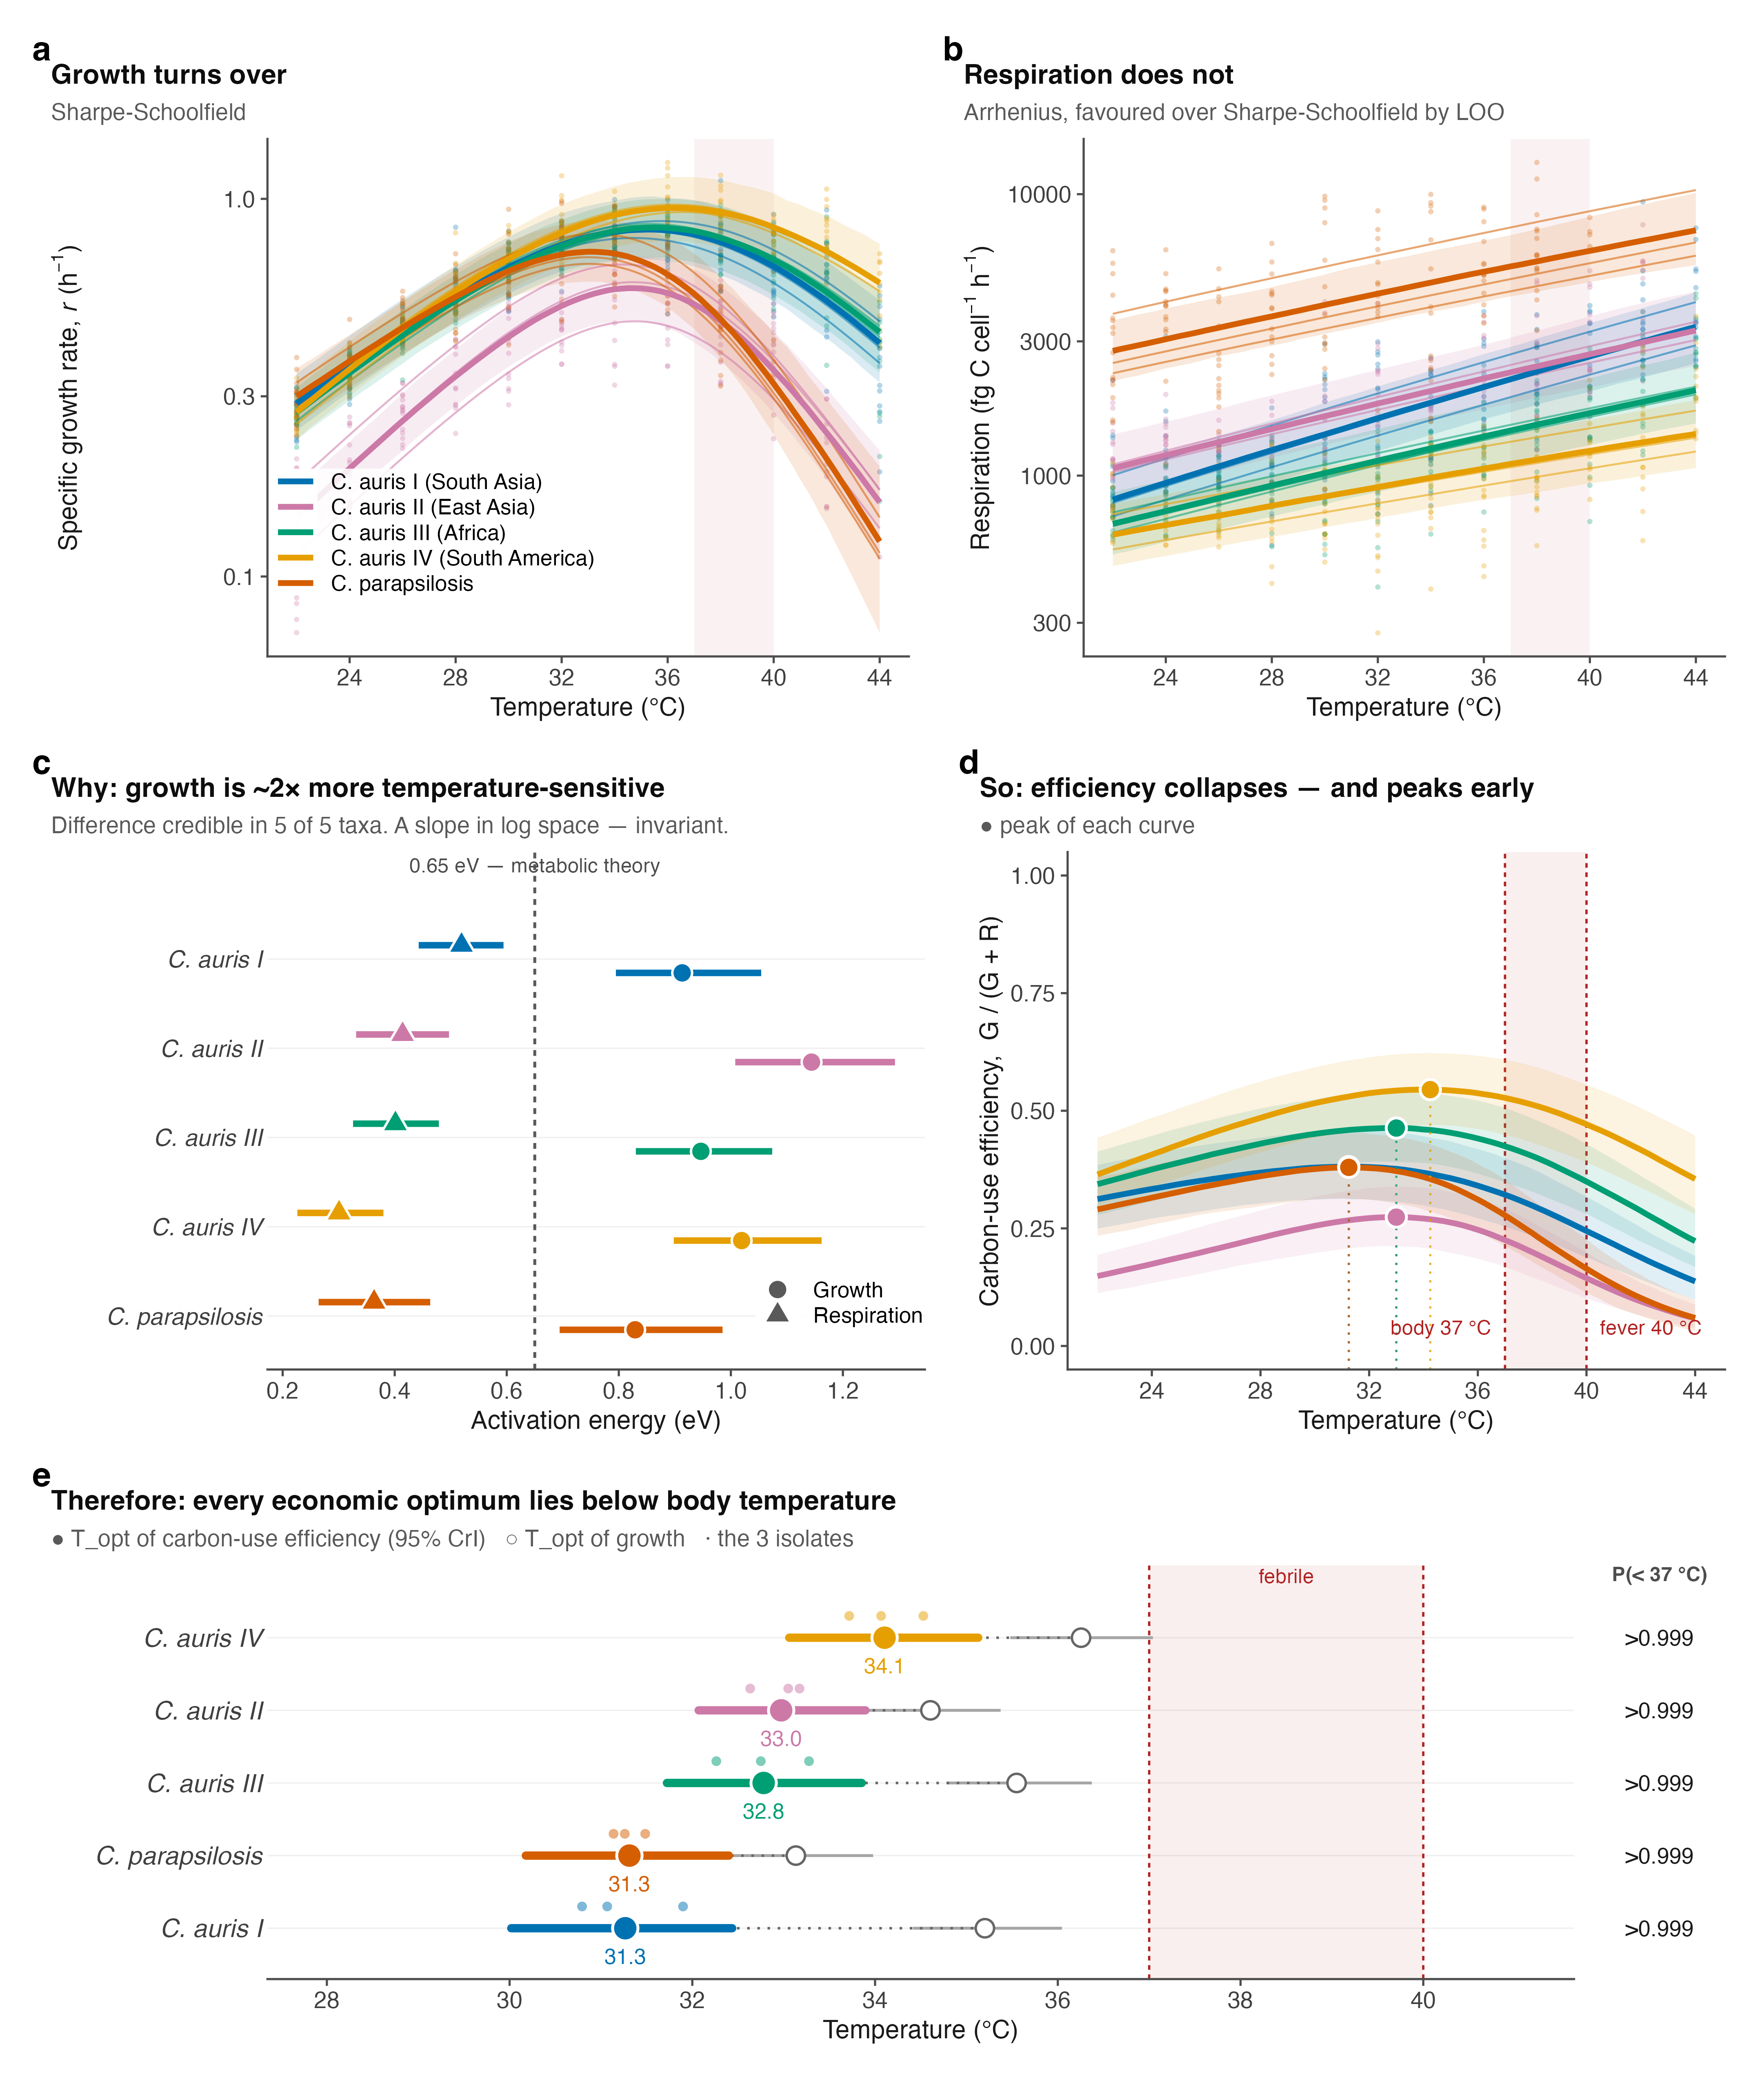
\includegraphics[width=1\linewidth,height=\textheight,keepaspectratio]{../../results/figures/manuscript/FIG1_decoupling.png}

\textbf{Figure 1. Growth and respiration decouple with temperature,
placing every carbon-economy optimum below body temperature.}
(\textbf{a}) Specific growth rate \emph{r} (h\textsuperscript{−1}) and
(\textbf{b}) per-cell respiration carbon flux (fg C
cell\textsuperscript{−1} h\textsuperscript{−1}) versus temperature
(points, isolate-level observations; thin lines, per-isolate fits; bold
lines, clade-level posterior medians; bands, 95\% CrI). Growth turns
over; respiration does not (Arrhenius favoured over Sharpe-Schoolfield
by leave-one-out cross-validation). (\textbf{c}) Activation energies of
growth (circles) and respiration (triangles); dashed line, the 0.65 eV
metabolic-theory value. Growth is credibly more temperature-sensitive
than respiration in all five taxa. (\textbf{d}) Carbon-use efficiency,
CUE = G/(G+R), collapses with warming and peaks early; filled points
mark each curve's peak. (\textbf{e}) Thermal optimum of CUE (filled
points, 95\% CrI; open points, growth optimum; small points, isolates),
with the posterior probability that it lies below 37 °C. Shaded band, 37
to 40 °C (body to fever).

\subsection{A febrile host imposes a quantifiable, taxon-specific carbon
tax}\label{a-febrile-host-imposes-a-quantifiable-taxon-specific-carbon-tax}

Because the economic optimum lies below 37 °C, every taxon operates at a
carbon penalty in the host. We express this as the relative respiratory
cost, i.e.~respiration per unit growth relative to each taxon's own
cheapest temperature (Fig. 2a). At 40 °C (fever), this cost reached
1.34× for \emph{C. auris} Clade IV but 3.13× for \emph{C. parapsilosis}.

The three-degree step from body temperature (37 °C) to fever (40 °C)
captures the clinical penalty most directly (Fig. 2c). Over this
interval \emph{C. parapsilosis} retained only 58\% of its 37 °C growth
rate (0.58, 95\% CrI 0.50-0.67) while its respiratory cost per unit
growth rose 1.96× (1.71-2.31). The \emph{C. auris} clades were far less
affected: Clade IV retained 89\% of growth (0.89, 0.85-0.93) at a cost
increase of only 1.25× (1.19-1.31), with Clades I-III intermediate
(growth retained 0.67-0.84; cost 1.37×-1.73×). Fever thus suppresses
growth without suppressing respiration, and it does so most severely in
\emph{C. parapsilosis}.

\textbf{A warmer environmental optimum predicts a lower cost of fever.}
Across the five taxa, the environmental growth optimum was strongly and
negatively associated with the metabolic cost of fever: the more
thermotolerant a taxon, the less a fever cost it (Fig. 2b). Computed as
a posterior distribution over Spearman's ρ (propagating parameter
uncertainty rather than treating the five taxon medians as fixed), the
correlation was ρ = −0.90 (95\% CrI −1.00 to −0.30; P(ρ \textless{} 0) =
0.996). \emph{C. parapsilosis} occupied the cool-optimum,
expensive-fever extreme and \emph{C. auris} Clade IV the warm-optimum,
cheap-fever extreme. This links adaptation to a warm environment with
tolerance of the febrile host as facets of a single thermal trait,
consistent with the hypothesis that environmental thermal selection
underlies fungal thermotolerance to the mammalian host. We note that
T\textsubscript{opt} and fever cost are partly geometrically coupled
through the growth curve; however, respiration (E\textsubscript{R}) is
an independent parameter that could have broken the relationship and did
not. The correlation rests on only five taxa; it is therefore reported
as suggestive and will be tested directly with additional species.

\textbf{Clade-level differences within \emph{C. auris}.} Pairwise
comparison of the fever cost resolved 8 of 10 taxon contrasts (95\% CrI
excluding a ratio of 1; Fig. 2d). All four \emph{C. auris} clades
credibly paid less at fever than \emph{C. parapsilosis} (cost ratios
0.43-0.72), and Clade IV was credibly the cheapest of all clades. Only
two contrasts, Clade I versus Clade II (0.85, 0.68-1.04) and Clade I
versus Clade III (1.18, 0.98-1.42), could not be separated at three
isolates per clade.

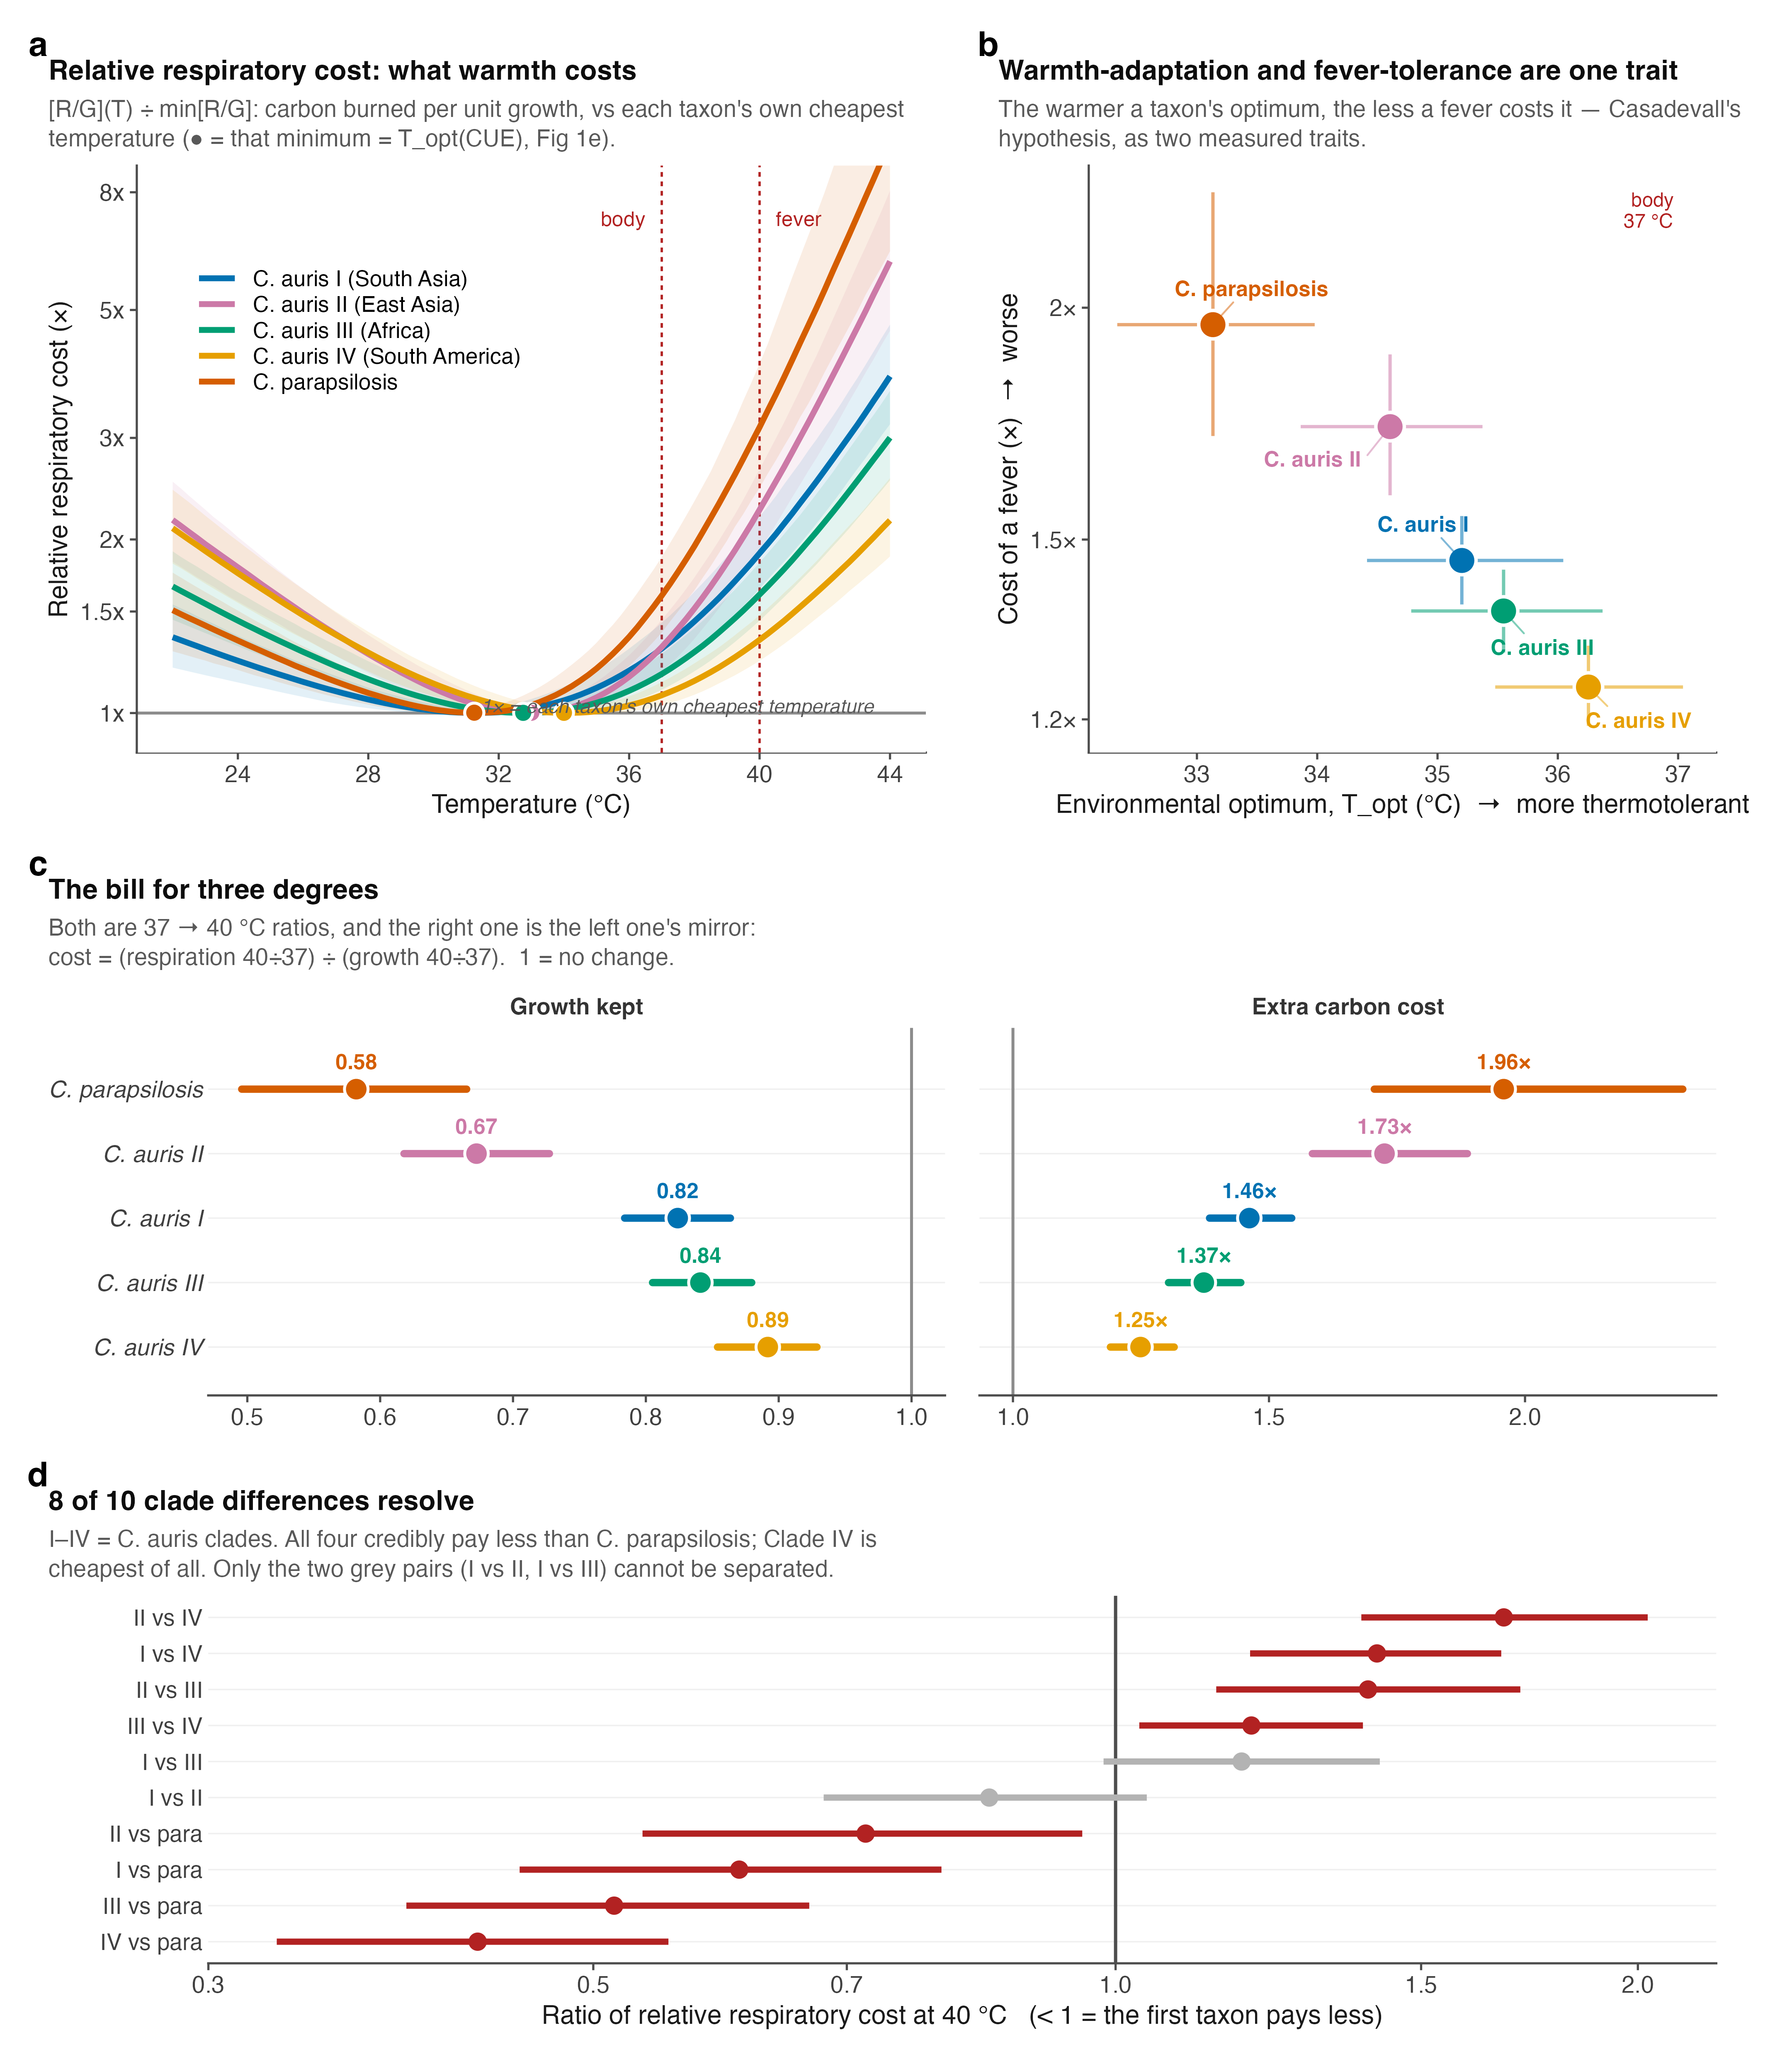
\includegraphics[width=1\linewidth,height=\textheight,keepaspectratio]{../../results/figures/manuscript/FIG2_the_bill.png}

\textbf{Figure 2. A febrile host imposes a quantifiable, taxon-specific
carbon tax.} (\textbf{a}) Relative respiratory cost (per-cell
respiration per unit growth, expressed relative to each taxon's own
cheapest temperature) versus temperature (bold lines, clade-level
posterior medians; bands, 95\% CrI). At 40 °C (fever) this cost ranged
from 1.34× for \emph{C. auris} Clade IV to 3.13× for \emph{C.
parapsilosis}. Shaded band, 37--40 °C (body to fever). (\textbf{b})
Environmental growth optimum versus the metabolic cost of fever across
the five taxa: warmer-adapted taxa pay less at fever (Spearman ρ =
−0.90, 95\% CrI −1.00 to −0.30; points, taxon medians; bars, 95\% CrI).
(\textbf{c}) The three-degree step from body temperature (37 °C) to
fever (40 °C): growth retained (left) and the rise in respiratory cost
per unit growth (right) for each taxon (points, posterior medians; bars,
95\% CrI). (\textbf{d}) Pairwise contrasts of the 40 °C fever cost; 8 of
10 are resolved (95\% CrI excluding a ratio of 1), and all four \emph{C.
auris} clades pay credibly less than \emph{C. parapsilosis}.

\subsection{Clade thermotolerance is a growth-tunable trait, not a
sequence
difference}\label{clade-thermotolerance-is-a-growth-tunable-trait-not-a-sequence-difference}

The respirometry establishes that the four \emph{C. auris} clades differ
roughly two-fold in peak growth, and correspondingly in their cost of
fever, despite being almost identical in coding sequence. We therefore
asked how much of this thermal physiology can be read from the genome
itself. To do so we built a sequence-grounded, enzyme- and
temperature-constrained genome-scale model (etc-GEM), which derives each
enzyme's molecular weight, turnover and thermal stability from its
protein sequence and predicts growth at every temperature under a shared
enzyme budget, with three physiological parameters calibrated to the
measured curve (Fig. 3). Every clade-specific input is sequence-derived,
so the model sees a clade only through its proteome. That makes it a
direct test of how far genomic data alone carries: if the clade
differences are written into coding sequence, the model should generate
them unaided.

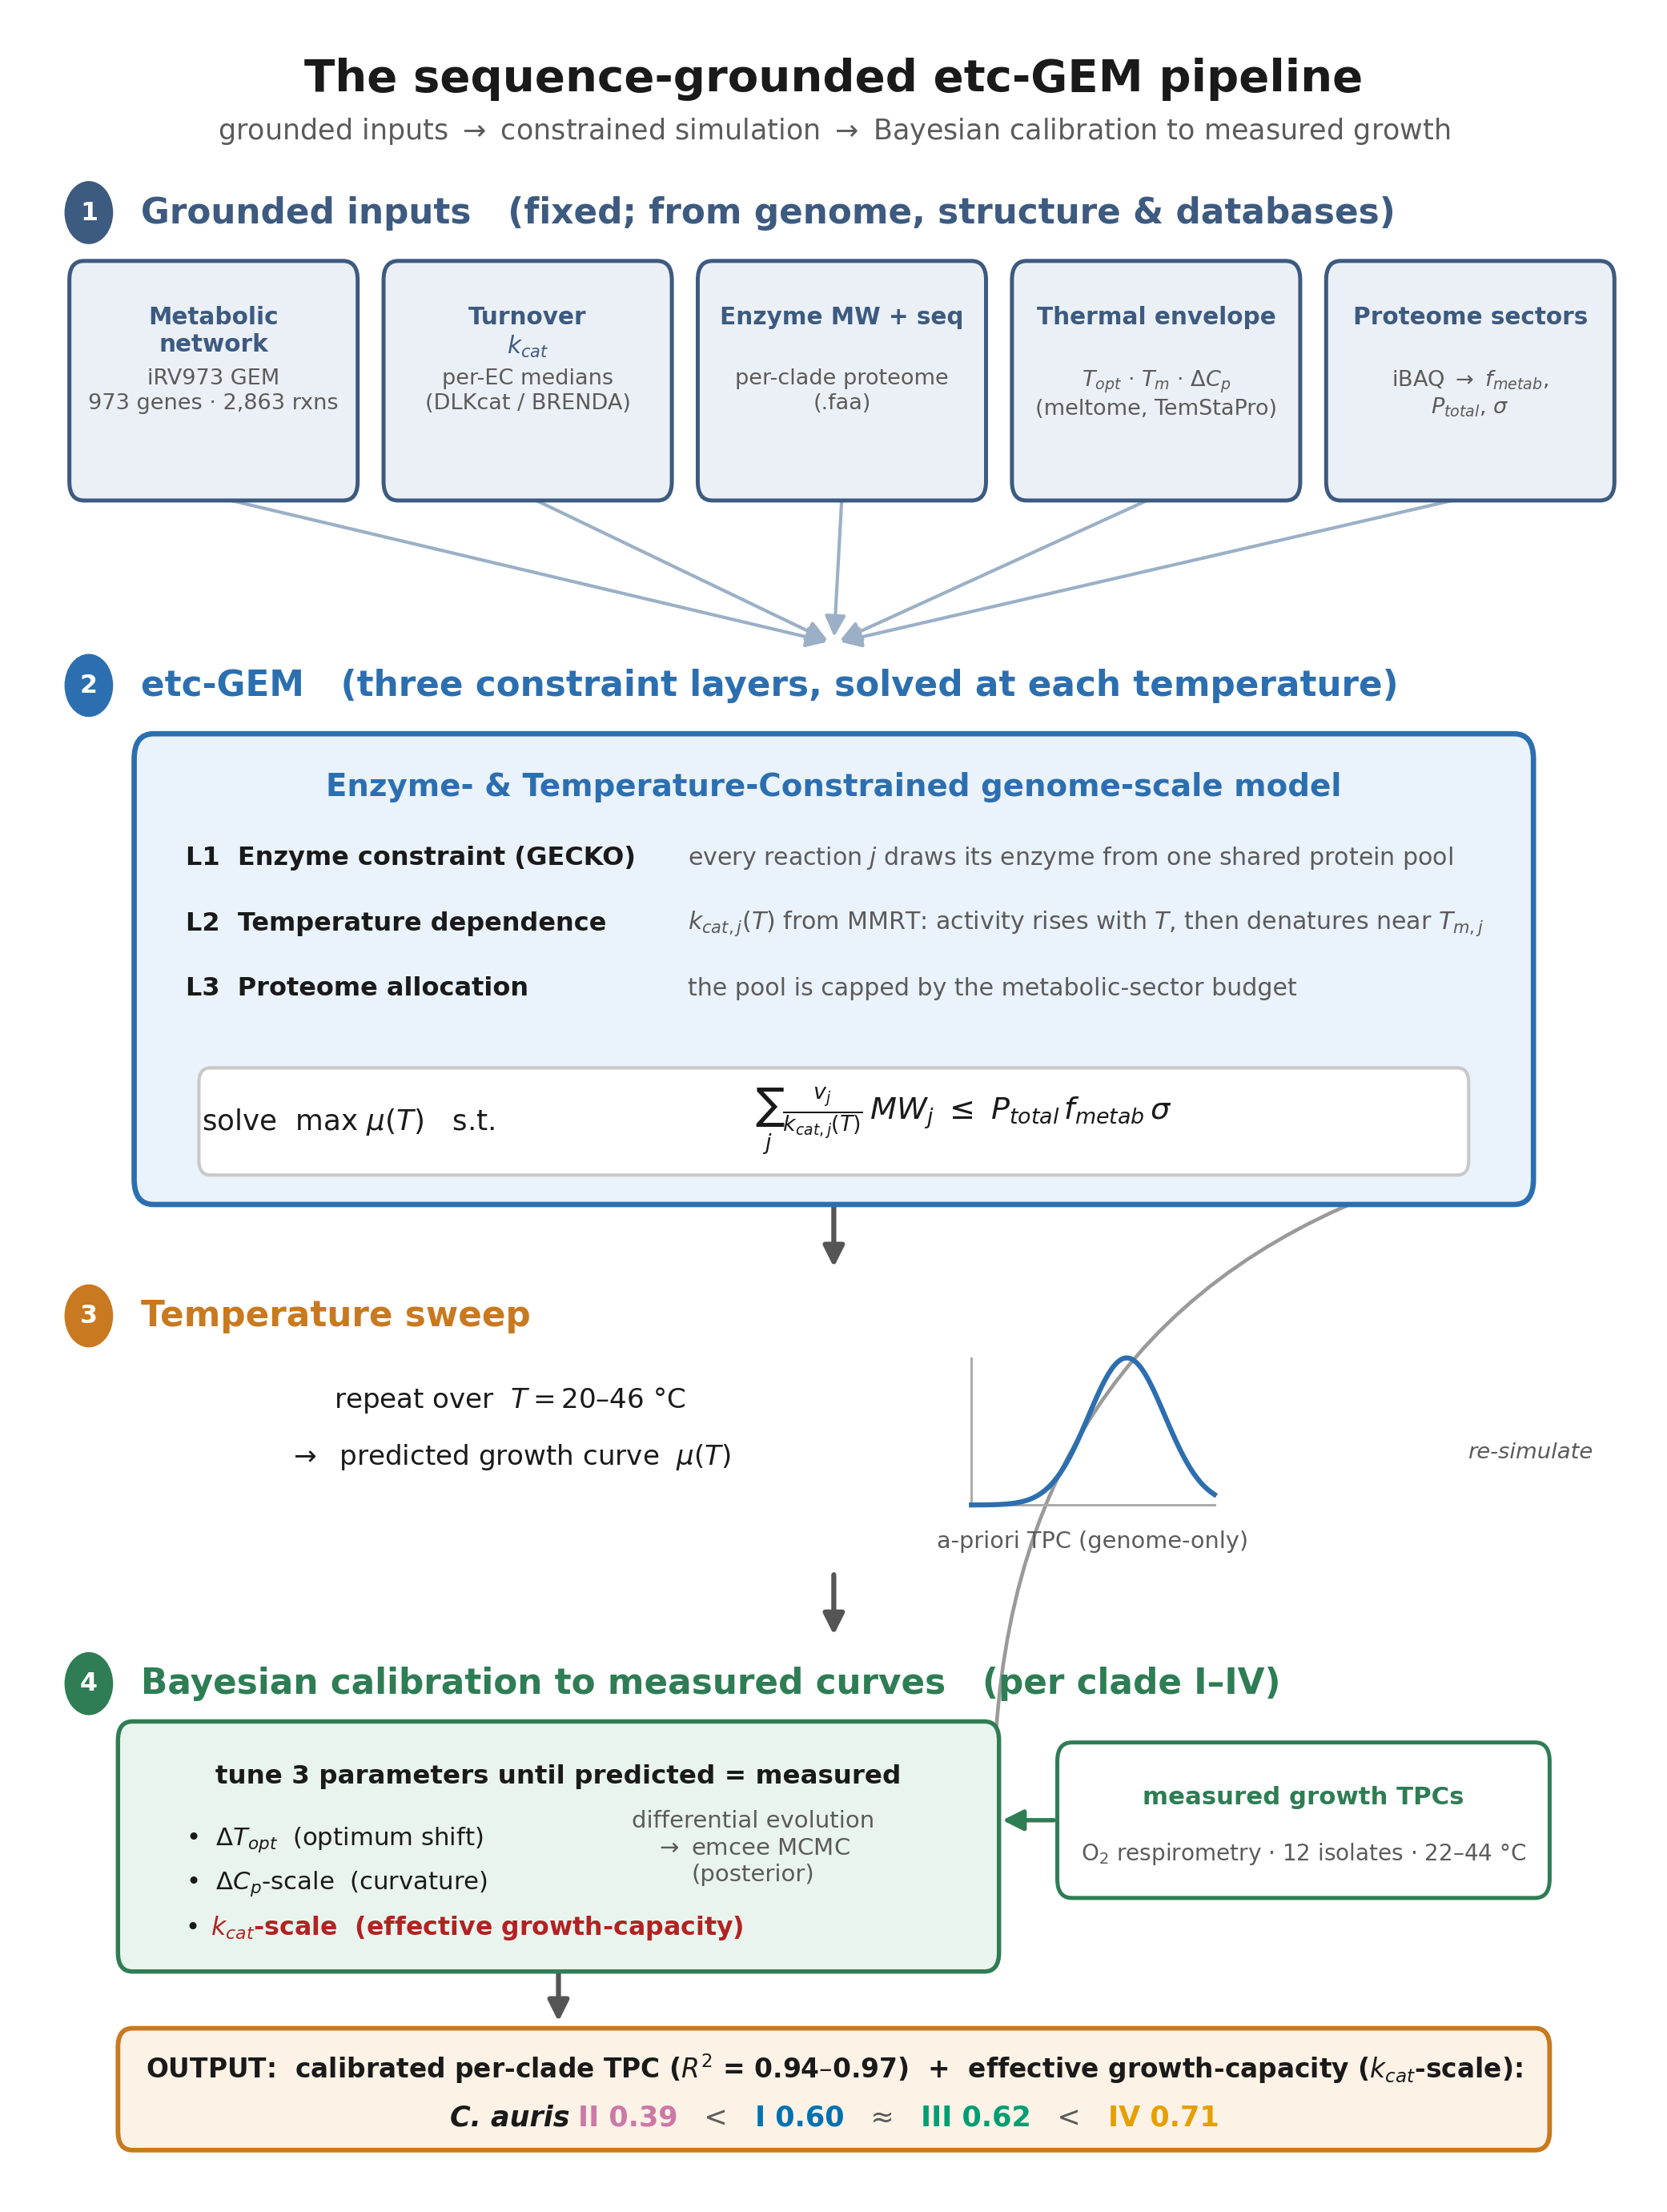
\includegraphics[width=1\linewidth,height=\textheight,keepaspectratio]{../../results/figures/manuscript/FIG_model_schematic.png}

\textbf{Figure 3. The sequence-grounded etc-GEM pipeline.} Fixed,
genome-derived inputs (the iRV973 metabolic network; per-reaction
turnover kcat from EC/DLKcat; enzyme molecular weights and per-clade
sequences; per-enzyme thermal parameters Topt, Tm and ΔCp; and
proteome-sector fractions) feed an enzyme- and temperature-constrained
genome-scale model that, at each temperature, maximises growth subject
to a shared enzyme budget. Three parameters (ΔTopt, ΔCp-scale, and
effective-capacity kcat-scale) are then calibrated by differential
evolution and MCMC to each clade\textquotesingle s measured growth
curve. Because the genome is \textgreater99\% identical across clades,
only the effective growth-capacity axis differs, giving the per-clade
values in Figure 4.

The four clades are near-identical at the enzyme level: median
whole-proteome amino-acid identity was 99.4-100\% across clades I-IV
(reciprocal best-hit alignment of the four reference proteomes).
Consequently the genome-derived model predicts a single, essentially
identical thermal curve for all four clades, whereas the measured clades
differ roughly two-fold in peak growth (Fig. 4b). Sequence variation
therefore cannot account for the clade differences. A per-clade
calibration nonetheless recovers each measured growth curve (Fig. 4a).

The difference resides instead in an effective growth-capacity axis
(kcat-scale), an effective flux-generating capacity per unit modelled
metabolic proteome that lumps enzyme abundance, active fraction,
substrate saturation, maintenance and respiratory coupling (Fig. 4c). It
is a single proteome-wide capacity scaling, not a change in the
individual database-derived kcat values, which are shared across the
near-identical clades. Its posterior ordered with thermotolerance (Clade
II lowest at 0.39, Clades I and III intermediate at 0.60 and 0.62, Clade
IV highest at 0.71), and of the three calibration parameters it was the
only one that separated the clades (5 of 6 pairwise contrasts with
non-overlapping 95\% CrI, versus 1 of 6 for the optimum shift and 0 of 6
for curvature; Supplementary Fig. 1b).

\textbf{The effective capacity axis covaries with measured respiratory
economics.} The growth-fitted effective-capacity scalar covaried across
the twelve isolates with independently measured, respiration-containing
outcomes. It was negatively associated with the cost of a fever (r =
-0.86, 95\% CI -0.96 to -0.76): the higher a clade\textquotesingle s
capacity, the cheaper its fever (Fig. 4d). It was likewise negatively
associated with per-cell respiration at the growth optimum (r = -0.64),
so that higher-capacity clades sustain growth while respiring less
carbon (Fig. 4e). These cross-phenotype associations indicate that the
scalar captures a reproducible physiological axis extending beyond
peak-growth amplitude, but they do not constitute independent
mechanistic validation of enzyme abundance. The fever tax is itself
derived from measured growth and respiration through carbon-use
efficiency, so it is not a fully independent target; and a
flux-variability analysis showed that oxygen consumption at fixed
optimal growth is not uniquely determined by the growth-calibrated
model, so the model\textquotesingle s respiration is an
objective-selected flux solution rather than a unique prediction.
Growth-only fits of alternative capacity, maintenance and uptake
constraints each reproduced the clade growth ranking but none recovered
the observed ranking in respiratory cost, and Clade II combined the
lowest growth with the highest respiratory cost. We therefore read the
fitted parameter as an effective growth-capacity axis that does not by
itself distinguish reduced enzyme deployment from a coupling or
maintenance component. Capacity behaved as a clade-level trait, with
90\% of its variance between clades (ICC\textsubscript{1} = 0.90; ANOVA
F\textsubscript{3},\textsubscript{8} = 27.7, P =
1.4×10\textsuperscript{−4}; Supplementary Fig. 1a). The
capacity-versus-peak-growth relationship, by contrast, is a
self-consistency check rather than independent evidence, because
capacity is itself the fitted height term (Supplementary Fig. 2).

Because the clades are near-identical in coding sequence, the capacity
differences cannot be encoded there. A direct transcriptional test did
not, however, localise them to bulk mRNA: in the only public
clade-resolved RNA-seq at a controlled condition (Clade I versus Clade
II, 37 °C; GEO GSE165762), the model\textquotesingle s 928
central-metabolic enzyme genes were not coordinately lower in the
low-capacity clade (median log\textsubscript{2} fold-change -0.005
versus +0.031 for the genome background; Wilcoxon P = 0.93;
Supplementary Fig. 1d). Because that analysis is compositional (standard
library-size-normalised RNA-seq, a single Clade II isolate, one 37 °C
snapshot), it rules out a relative down-allocation of metabolic
transcripts, not lower absolute output. The causal layer is therefore
non-coding, regulatory, post-transcriptional, post-translational, or
bioenergetic, and remains undetermined among these; distinguishing them
will require a model-identifiability analysis (profiling capacity
against maintenance, uptake and respiratory coupling) together with
absolute, spike-in-calibrated proteomics, which partitions but does not
fully close these branches.

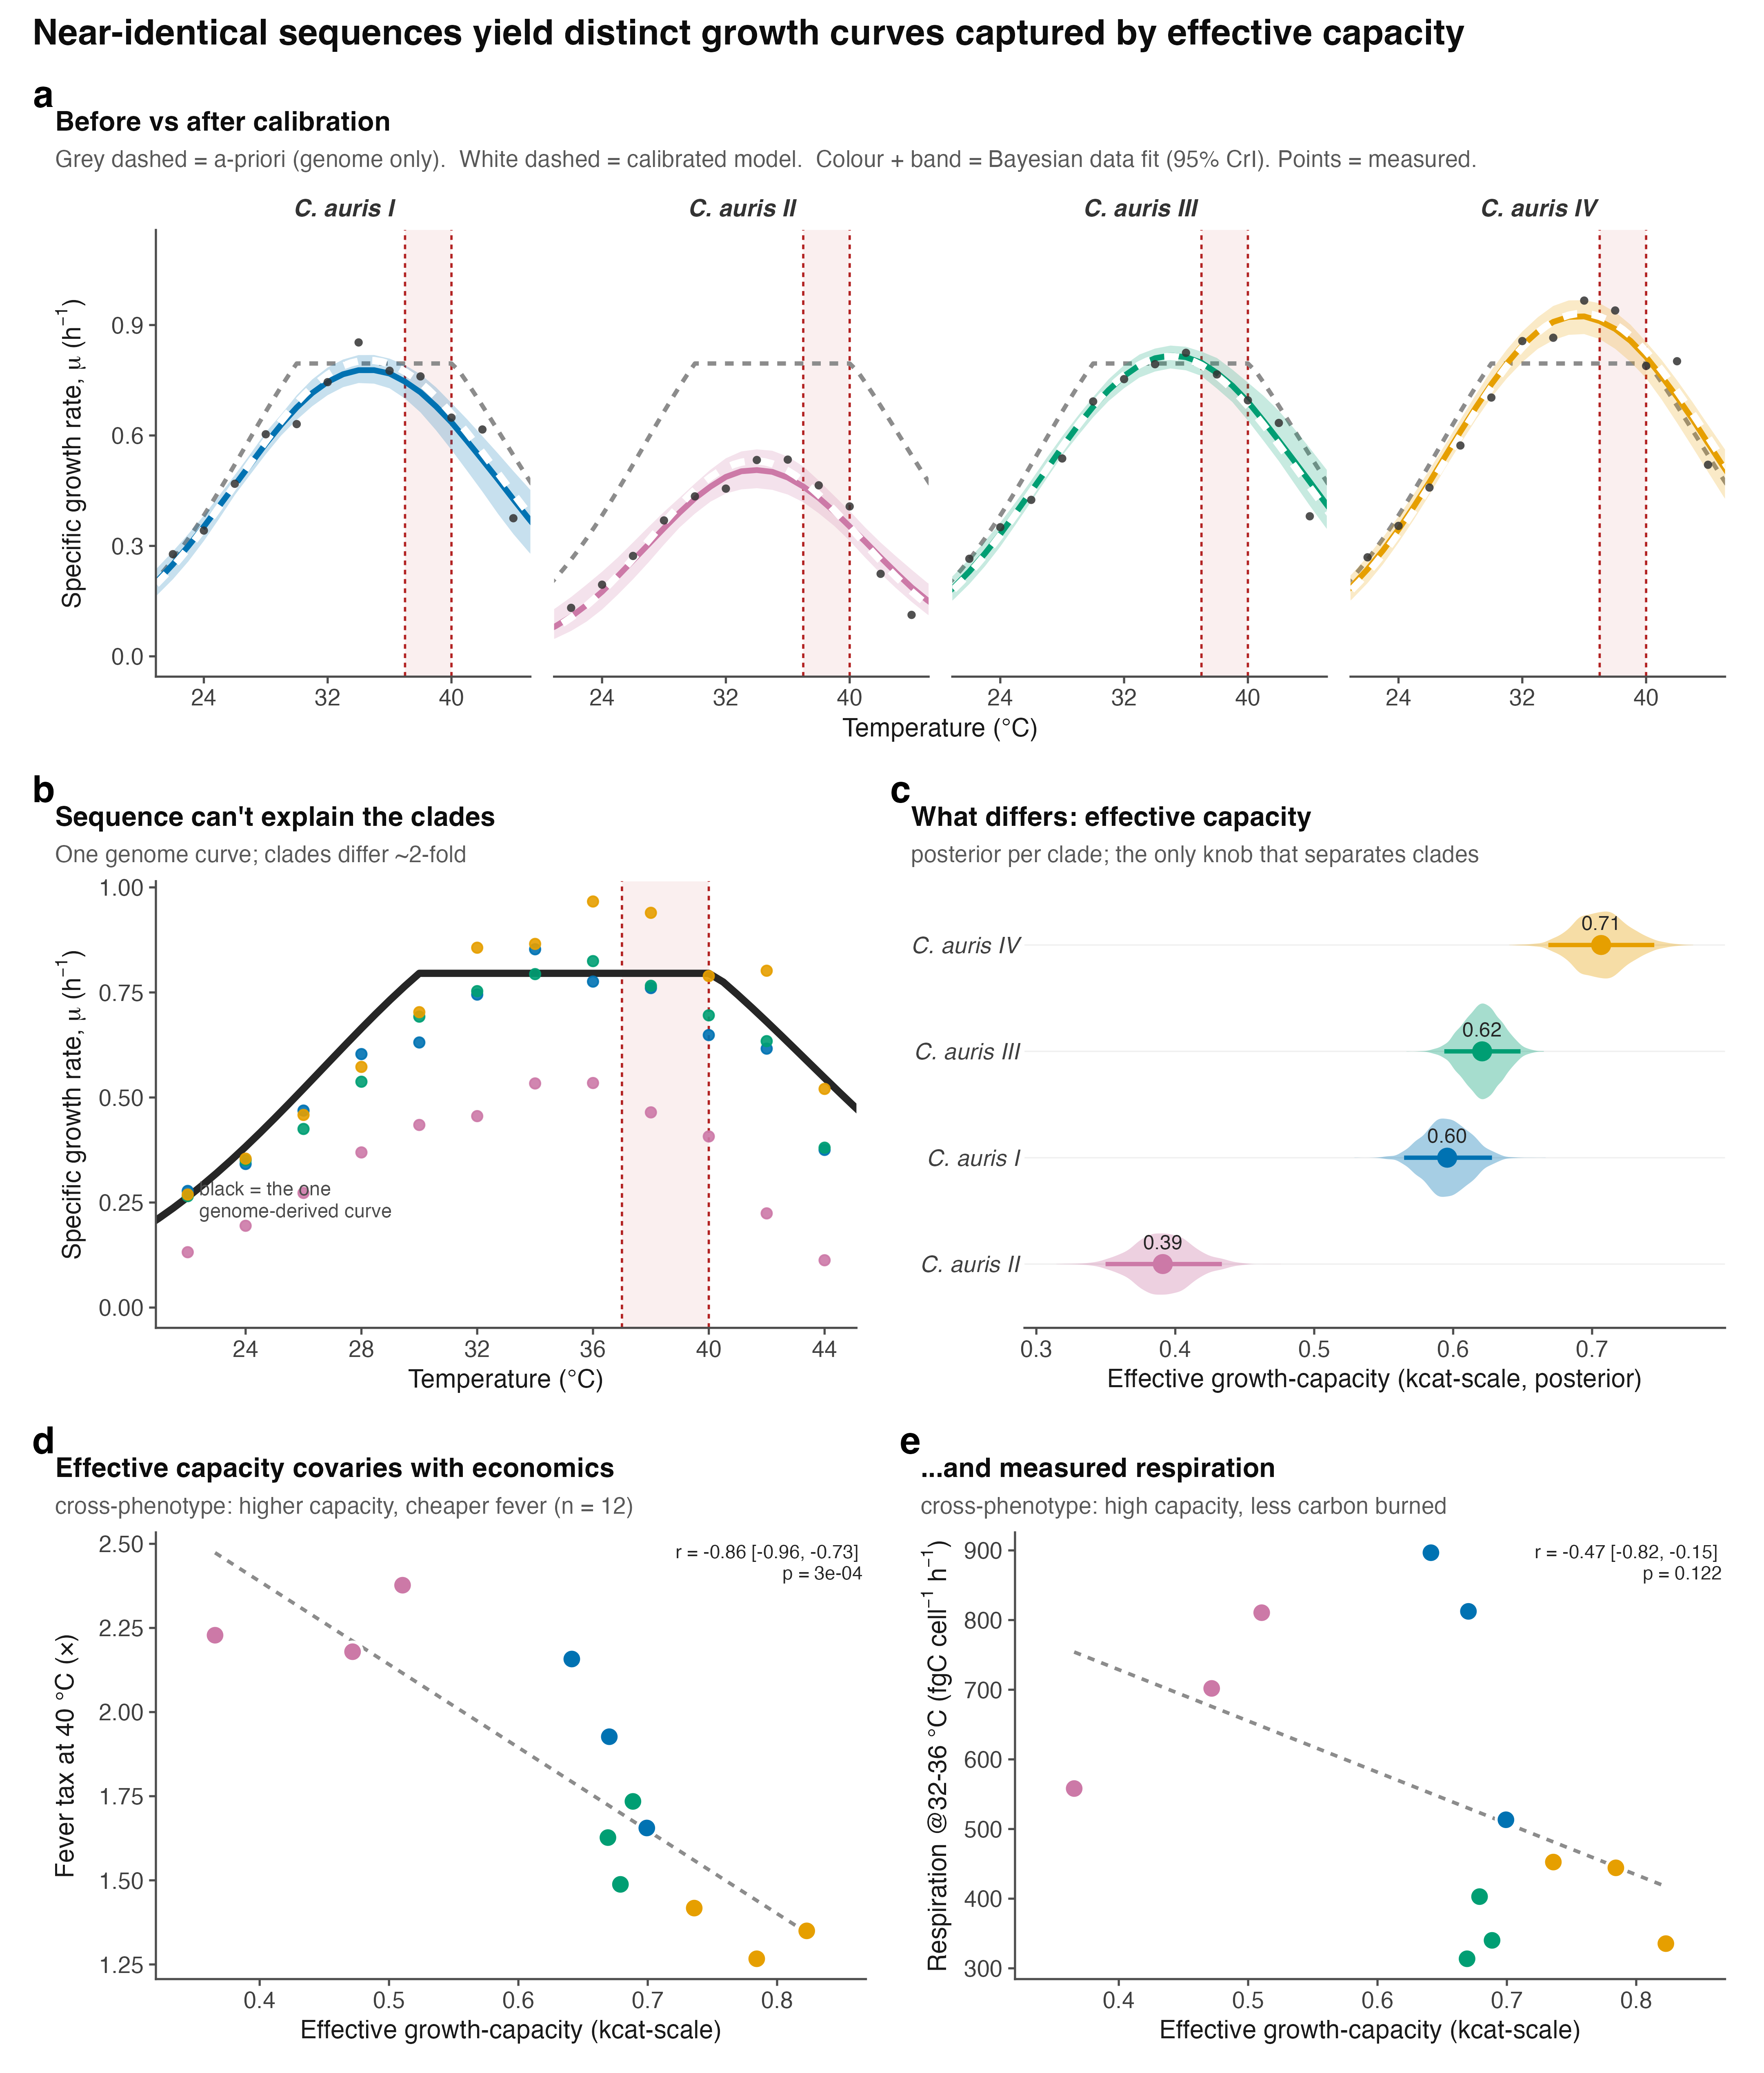
\includegraphics[width=1\linewidth,height=\textheight,keepaspectratio]{../../results/figures/manuscript/FIG_MODEL.png}

\textbf{Figure 4. Clade thermotolerance is a growth-tunable trait, not
sequence.} (\textbf{a}) Per-clade calibration of the sequence-grounded
etc-GEM: grey dashed, genome-only (a-priori) prediction; white dashed,
calibrated model; colour and band, Bayesian data fit (95\% CrI); points,
measured. (\textbf{b}) The genome yields one curve for all clades
(black), yet the measured clades differ \textasciitilde2-fold.
(\textbf{c}) Posterior of the effective growth-capacity parameter
(kcat-scale) per clade; the only calibration parameter that separates
the clades. (\textbf{d}) Effective growth-capacity versus the measured
fever tax at 40 °C and (\textbf{e}) versus per-cell respiration at 32-36
°C (points, twelve isolates coloured by clade). The scalar was fitted to
growth only; d-e are cross-phenotype associations, not independent
mechanistic validation, because the fever tax derives from measured
growth and respiration and the model\textquotesingle s respiration at
fixed growth is not uniquely determined (see text). They replace the
earlier capacity-versus-growth panel, which was a self-consistency check
(Supplementary Fig. 2).

\section{References}\label{references}

\protect\phantomsection\label{refs}
\begin{CSLReferences}{0}{0}
\bibitem[\citeproctext]{ref-cakin2026}
\CSLLeftMargin{1. }%
\CSLRightInline{Cakin, I. \emph{et al.}
\href{https://doi.org/10.1093/ismeco/ycag024}{A novel method to
simultaneously estimate bacterial respiration and growth from oxygen
dynamics}. \emph{ISME Communications} \textbf{6}, ycag024 (2026).}

\bibitem[\citeproctext]{ref-viana2023}
\CSLLeftMargin{2. }%
\CSLRightInline{Viana, R. \emph{et al.}
\href{https://doi.org/10.1093/femsyr/foad045}{Metabolic reconstruction
of the human pathogen {Candida} auris: Using a cross-species approach
for drug target prediction}. \emph{FEMS Yeast Research} \textbf{23},
foad045 (2023).}

\bibitem[\citeproctext]{ref-Li2021}
\CSLLeftMargin{3. }%
\CSLRightInline{Li, G. \emph{et al.}
\href{https://doi.org/10.1038/s41467-020-20338-2}{Bayesian genome scale
modelling identifies thermal determinants of yeast metabolism}.
\emph{Nature Communications} \textbf{12}, 190 (2021).}

\bibitem[\citeproctext]{ref-yvondurocher_etcgem}
\CSLLeftMargin{4. }%
\CSLRightInline{{Yvon-Durocher, G. \emph{et al.}} {etcGEMs}: An enzyme-
and temperature-constrained genome-scale modelling pipeline. (2024).}

\bibitem[\citeproctext]{ref-Madkaikar2023}
\CSLLeftMargin{5. }%
\CSLRightInline{Madkaikar, A. Predicting the temperature dependence of
microbial metabolism with enzyme- and temperature-constrained
genome-scale models. (Imperial College London, 2023).}

\bibitem[\citeproctext]{ref-Domenzain2022}
\CSLLeftMargin{6. }%
\CSLRightInline{Domenzain, I. \emph{et al.}
\href{https://doi.org/10.1038/s41467-022-31421-1}{Reconstruction of a
catalogue of genome-scale metabolic models with enzymatic constraints
using {GECKO} 2.0}. \emph{Nature Communications} \textbf{13}, 3766
(2022).}

\bibitem[\citeproctext]{ref-dlkcat2022}
\CSLLeftMargin{7. }%
\CSLRightInline{Li, F. \emph{et al.}
\href{https://doi.org/10.1038/s41929-022-00798-z}{Deep learning-based
{kcat} prediction enables improved enzyme-constrained model
reconstruction}. \emph{Nature Catalysis} \textbf{5}, 662--672 (2022).}

\bibitem[\citeproctext]{ref-LiEngqvist2019}
\CSLLeftMargin{8. }%
\CSLRightInline{Li, G., Rabe, K. S., Nielsen, J. \& Engqvist, M. K. M.
\href{https://doi.org/10.1021/acssynbio.9b00099}{Machine learning
applied to predicting microorganism growth temperatures and enzyme
catalytic optima}. \emph{ACS Synthetic Biology} \textbf{8}, 1411--1420
(2019).}

\bibitem[\citeproctext]{ref-Jarzab2020}
\CSLLeftMargin{9. }%
\CSLRightInline{{Jarzab, A., Kurzawa, N., \emph{et al.}}
\href{https://doi.org/10.1038/s41592-020-0801-4}{Meltome atlas---thermal
proteome stability across the tree of life}. \emph{Nature Methods}
\textbf{17}, 495--503 (2020).}

\bibitem[\citeproctext]{ref-Hobbs2013}
\CSLLeftMargin{10. }%
\CSLRightInline{Hobbs, J. K. \emph{et al.}
\href{https://doi.org/10.1021/cb4005029}{Change in heat capacity for
enzyme catalysis determines temperature dependence of enzyme catalyzed
rates}. \emph{ACS Chemical Biology} \textbf{8}, 2388--2393 (2013).}

\bibitem[\citeproctext]{ref-zamithmiranda2019}
\CSLLeftMargin{11. }%
\CSLRightInline{Zamith-Miranda, D. \emph{et al.}
\href{https://doi.org/10.1128/mSystems.00257-19}{Multi-omics signature
of {Candida} auris, an emerging and multidrug-resistant pathogen}.
\emph{mSystems} \textbf{4}, e00257--19 (2019).}

\bibitem[\citeproctext]{ref-Ebrahim2013}
\CSLLeftMargin{12. }%
\CSLRightInline{Ebrahim, A., Lerman, J. A., Palsson, B. O. \& Hyduke, D.
R. \href{https://doi.org/10.1186/1752-0509-7-74}{{COBRApy}:
{COnstraints}-{Based} {Reconstruction} and {Analysis} for {Python}}.
\emph{BMC Systems Biology} \textbf{7}, 74 (2013).}

\bibitem[\citeproctext]{ref-ForemanMackey2013}
\CSLLeftMargin{13. }%
\CSLRightInline{Foreman-Mackey, D., Hogg, D. W., Lang, D. \& Goodman, J.
\href{https://doi.org/10.1086/670067}{Emcee: The {MCMC} hammer}.
\emph{Publications of the Astronomical Society of the Pacific}
\textbf{125}, 306--312 (2013).}

\end{CSLReferences}




\end{document}
